% ===========================================================================
\section{Introduction}
\label{sec:introduction}
% ===========================================================================

Methane emissions from oil and natural-gas systems do not scale with production alone. They
arise from wells, tanks, compressors, processing plants, pipelines, distribution networks,
appliances and episodic releases; their magnitude depends on equipment and operating practice.
An inventory built only from national production therefore misses much of the source population
and obscures the infrastructure where mitigation would occur.

The distinction is methodological. The 2006 IPCC Guidelines published broad Tier~1 ranges for
developing-country systems, including ranges spanning orders of magnitude
\citep{ipcc2006fugitives}. The 2019 Refinement introduced separate factors for oil production,
transport and refining and for gas production, gathering, processing, transmission,
distribution and post-meter sources. Several factors depend explicitly on
leak-detection-and-repair (LDAR), pipeline material and compressor-seal practice
\citep{ipcc2019}. Applying the Refinement in a data-scarce country therefore requires both a
method change and a reconstruction of the physical supply chain.

Pakistan is a useful case. National production statistics are public, and the regulator reports
utility throughput, pipeline length, compressor infrastructure, customers, LNG terminals,
refinery production and unaccounted-for gas (UFG). Satellite-derived flare locations and
methane-plume detections provide independent spatial evidence. Pakistan's official reporting,
however, remains difficult to reconcile with these activity data, and direct national leakage
measurements are unavailable.

This study addresses three questions. First, how much of the difference between legacy and
refined fugitive estimates results from revised factors, and how much from adding previously
omitted supply-chain segments? Second, which unresolved infrastructure characteristics dominate
the national range? Third, what constraints are provided by utility balances, official reporting
and satellite observations?

We answer these questions with a conserved segment inventory and physical gas-flow account, a
method-resolution experiment, separate structural and parametric uncertainty analyses, and
matched official and observational evaluations. The same source-neutral ledger can accept
aggregate public controls today and facility-level records when they become available.
Figure~\ref{fig:framework} summarizes the workflow.

\begin{figure*}[htbp]
\centering
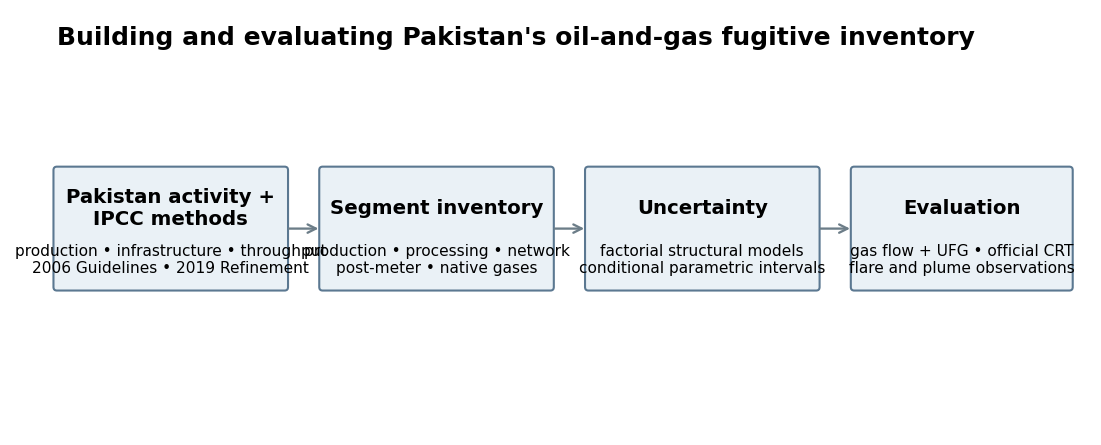
\includegraphics[width=0.90\textwidth]{fugitives_framework.png}
\caption{Scientific workflow from Pakistani activity data and IPCC methods through the segment
inventory, uncertainty analysis and three independent evaluation layers.}
\label{fig:framework}
\end{figure*}
